\documentclass[10pt,letterpaper]{article}
\usepackage[letterpaper,margin=0.75in]{geometry}
\usepackage[utf8]{inputenc}
\usepackage[russian,english]{babel}
\usepackage{mdwlist}
\usepackage[T2A]{fontenc}
\usepackage{textcomp}
\usepackage{tgpagella}
\usepackage{amsmath}
\usepackage{mathtools}
\usepackage{tikz}
\usepackage{tikz-3dplot}
\usepackage{caption}
\usepackage{subfig}
\usepackage{indentfirst}
\usepackage{listings}
\setlength{\tabcolsep}{2em}
\setlength{\parindent}{4em}
\setlength{\parskip}{1em}

\numberwithin{equation}{section}
\numberwithin{figure}{section}
\numberwithin{table}{section}
\renewcommand{\thesubfigure}{\thefigure.\arabic{subfigure}}
\captionsetup[subfigure]{labelformat=simple,labelsep=colon,listofformat=subsimple}

\title{Coordinates conversion in acoustic positioning}
\author{Oleksandr Novychenko}

\begin{document}

\maketitle

\section{General information}
During an acoustic positioning by ultra-short baseline transceiver a direction to a
target is measured as a round-trip time. When sound speed is known a distance between
USBL transceiver and transponder can be calculated. In combination with measured direction
it allows to calculate target coordinates in USBL-frame (or USBL-Frame) $\vec{X}_{ut}$
in \texttt{USBLLONG}.

In some scenarios USBL transceiver can't measure distance to target. In that case bearing
$\theta_{ut}$ and elevation $\varphi_{ut}$ angles are provided in \texttt{USBLANGLES}.
Covertion to USBL-Frame when distance $d$ is known is:
\begin{equation}
    \vec{X}_{ut} = d \cdot \begin{bmatrix}
        \sin \theta_{ut} \cos \varphi_{ut} \\
        \cos \theta_{ut} \cos \varphi_{ut} \\
        \sin \varphi_{ut}
    \end{bmatrix}
\end{equation}

USBL-Frame corrdinates $\vec{X}_{ut}$ should be converted to Vessel-Frame coordinates
$\vec{X}_vt$ by correction to USBL location $\vec{X}_{vu}$ and rotation $[R_{vu}]$:
\begin{equation}
    \vec{X}_{vt} = \vec{X}_{vu} + [R_{vu}] \cdot \vec{X}_{ut}.
    \label{equ:lf2vf}
\end{equation}

Vessel-Frame coordinates of target $\vec{X}_{vt}$ could be motion-compensated by using
information about attitude and heading of a vessel $[R_{vn}]$. Let $\varphi_{vn}$ (roll), $\theta_{vn}$
(pitch) and $\psi_{vn}$ (yaw) angles are provided by vessels AHRS. As result Topocentric
coordinates (North-East-Down) with Vessel-Frame origin are computed:
\begin{equation}
    \vec{N}_{vt} = [R_{vn}] \cdot \vec{X}_{vt}
    \label{equ:vf2ned}
\end{equation}

When Geodetic coordinates of Vessel-Frame origin $\vec{G}_{v}$ and Topocentric coordinates
of target $\vec{N}_{vt}$ are known, Geodetic coordinates of target $\vec{G}_{t}$ can be
computed.


\section{Definitions}

\subsection{Coordinate systems}
Vessel-Frame is cartesian coordinate system with origin somewere on a vessel. Usually on
stern. $X_{v}$-axis is directed forward, $Y_{v}$-axis directed astarboard and $Z_{v}$-axis
is directed down by right-hand rule.

USBL-Frame coordinate system has origin in the middle of USBL transceiver. $Y_{u}$-axis
is directed to white mark on USBL-head (forward), $Z_{u}$-axis is directed to subconn port
direction (up) and $X_{u}$ by right-hand rule directs right.

\begin{figure}
    \centering
    \tdplotsetmaincoords{70}{30}
    \begin{tikzpicture}[scale=5,tdplot_main_coords]
        \coordinate (O) at (0,0,0);
        \coordinate (U) at (0.1,0.03,-0.15);

        \draw[] (0,0,0) node[anchor=south east]{$O$};
        \draw[thick,->] (0,0,0) -- (0,1,0) node[anchor=south west]{$X_{v}$};
        \draw[thick,->] (0,0,0) -- (1,0,0) node[anchor=north west]{$Y_{v}$};
        \draw[thick,->] (0,0,0) -- (0,0,-0.75) node[anchor=north]{$Z_{v}$};

        \draw[thin,dashed,->] (O) -- (U) node[anchor=north]{$\vec{X}_{vu}$};

        \tdplotsetrotatedcoordsorigin{(U)};
        \draw[dotted,tdplot_rotated_coords,->] (0,0,0) -- (0.5,0,0);
        \draw[dotted,tdplot_rotated_coords,->] (0,0,0) -- (0,0.5,0);
        \draw[dotted,tdplot_rotated_coords,->] (0,0,0) -- (0,0,0.5);

        \tdplotsetrotatedcoords{-15}{5}{0};
        \draw[thick,tdplot_rotated_coords,->] (0,0,0) -- (0.5,0,0) node[anchor=west]{$X_{u}$};
        \draw[thick,tdplot_rotated_coords,->] (0,0,0) -- (0,0.5,0) node[anchor=south]{$Y_{u}$};
        \draw[thick,tdplot_rotated_coords,->] (0,0,0) -- (0,0,0.5) node[anchor=west]{$Z_{u}$};
    \end{tikzpicture}
    \caption{USBL-Frame located in Vessel-Frame}
    \label{pic:devcrf}
\end{figure}


\subsection{Rotation}
Rotation of coordinates around speceific axis on specific angle could be done by using
Quaternions or Direction-Cosine Matrices (or Rotation Matrices).

Quaternions allows to apply rotation around arbitary axes. Positive direction of rotation
is a clockwise rotation when watching towards the axis. DCM allows the same, but its
more intuitive to describe vector operations with it.

Multiplying rotation Matrix to a column vector produces rotated column vector.

DCM can be built from quaternion in case of arbitary axis $\vec{r}$ and angle $\Omega$ or
as a combination of rotations around $X$, $Y$ and $Z$ axes (in $X-Y-Z$ order).

Angles $\varphi$, $\theta$ and $\psi$ are also known as Euler angles. Rotation matrix
$[R(\varphi, \theta, \psi)] = [R_{z}(\psi)] \cdot [R_{y}(\theta)] \cdot [R_{x}(\varphi)]$.

Applying rotation $[R_{ab}]$ and shift $\vec{X}_{ab}$ to point $\vec{X}_{a}$:
\begin{equation}
    \begin{bmatrix}
        x_{b} \\ y_{b} \\ z_{b}
    \end{bmatrix} = \begin{bmatrix}
        x_{ab} \\ y_{ab} \\ z_{ab}
    \end{bmatrix} + \begin{bmatrix}
         \cos \psi_{ab}   & -\sin \psi_{ab}    & 0                  \\
         \sin \psi_{ab}   &  \cos \psi_{ab}    & 0                  \\
        0                 & 0                  & 1
    \end{bmatrix} \cdot \begin{bmatrix}
         \cos \theta_{ab} & 0                  &  \sin \theta_{ab}  \\
        0                 & 1                  & 0                  \\
        -\sin \theta_{ab} & 0                  &  \cos \theta_{ab}
    \end{bmatrix} \cdot \begin{bmatrix}
        1                 & 0                  & 0                  \\
        0                 &  \cos \varphi_{ab} & -\sin \varphi_{ab} \\
        0                 &  \sin \varphi_{ab} &  \cos \varphi_{ab}
    \end{bmatrix} \cdot \begin{bmatrix}
        x_{a} \\ y_{a} \\ z_{a}
    \end{bmatrix}.
    \label{equ:rot_xyz}
\end{equation}

\begin{figure}
    \centering
    \tdplotsetmaincoords{60}{30}
    \begin{tikzpicture}[scale=5,tdplot_main_coords]
        \draw[] (0,0,0)  node[anchor=east]{$O$};
        \draw[thick,->] (0,0,0) -- (1,0,0) node[anchor=north west]{$X$};
        \draw[thick,->] (0,0,0) -- (0,1,0) node[anchor=south west]{$Y$};
        \draw[thick,->] (0,0,0) -- (0,0,1) node[anchor=south]{$Z$};

        \tdplotsetrotatedcoords{0}{90}{0};
        \tdplotdrawarc[thin,tdplot_rotated_coords,->]{(0,0,0.66)}{0.1}{0}{270}{anchor=south}{$\varphi$};

        \tdplotsetrotatedcoords{90}{90}{60};
        \tdplotdrawarc[thin,tdplot_rotated_coords,->]{(0,0,0.66)}{0.1}{0}{270}{anchor=south}{$\theta$};

        \tdplotsetrotatedcoords{90}{0}{90};
        \tdplotdrawarc[thin,tdplot_rotated_coords,->]{(0,0,0.66)}{0.1}{0}{270}{anchor=north west}{$\psi$};
    \end{tikzpicture}
    \caption{Euler angles}
    \label{pic:euler}
\end{figure}

Single forlmula to computation rotation matrix (\ref{equ:rot_xyz}) from Euler angles:
\begin{equation}
    [R(\varphi, \theta, \psi)] = \begin{bmatrix}
        \cos \theta \cos \psi &
        \sin \varphi \sin \theta \cos \psi - \cos \varphi \sin \psi &
        \cos \varphi \sin \theta \cos \psi + \sin \varphi \cos \psi \\
        \cos \theta \sin \psi &
        \sin \varphi \sin \theta \sin \psi + \cos \varphi \cos \psi &
        \cos \varphi \sin \theta \sin \psi - \sin \varphi \cos \psi \\
        -\sin \theta &
        \sin \varphi \cos \theta &
        \cos \varphi \cos \theta
    \end{bmatrix}.
    \label{equ:rpy2dcm}
\end{equation}

Angles can be extracted from DCM by:
\begin{equation}
    \begin{split}
        \varphi & = \arctg R_{32} / R_{33}, \\
        \theta  & = -\arcsin R_{31}, \\
        \psi    & = \arctg R_{21} / R_{11}.
    \end{split}
    \label{equ:dcm2rpy}
\end{equation}

DCMs has a property: $[R]^{-1} = [R]^{T}$.

From physical point of view, $\varphi$, $\theta$ and $\psi$ angles are also called as
Roll, Pitch and Yaw. Usually AHRS sensors provides angles for NED-frame: Roll --- port up,
Pitch --- bow up, Yaw --- heading for Vessel-Frame specified earlier.


\section{Coordinates convertion}


\subsection{Topocentric coordinates}

As mentioned in (\ref{equ:lf2vf}) an offset and rotation of USBL relaive to
Vessel-frame is required.

It is possible that AHRS sensor located with some bias $[R_{va}]$. In this case
Euler angles (or rotation matrix $[R_{an}]$) convertion is needed.

As mentionoed in (\ref{equ:vf2ned}), coordinates in AHRS-Frame can be converted
to $NED$ by multiplication to $[R_{vn}]$. To convert coordinates from Vessel-Frame
to AHRS Frame a multiplication to $[R_{va}]^{-1}$ is needed.

Inverted DCM $[R_{va}]^{-1}$ has an easy explanation. Since $[R_{vu}]$ (USBL-Frame
rotation) and $[R_{va}]$ (AHRS-Frame rotation) are both specified in Vessel-Frame,
first is used to convert $USBL \rightarrow VF$, second for $AHRS \rightarrow VF$.
Since transformation $VF \rightarrow AHRS$ is needed, rotation matrix is inverted.
\begin{equation}
    [R_{vn}] = [R_{an}] \cdot [R_{va}]^{-1}
\end{equation}


\subsection{Geographic coordinates}

When GNSS is used, geodetic coordinates $\vec{G}_{g}$ of antenna (which is
located at $\vec{X}_{vg}$ in Vessel-Frame) are measured:
\begin{equation}
    \vec{G} = [ \varphi, \lambda, h ]^{T}
\end{equation}

Geogetic Latitude $\varphi$ and Longitude $\lambda$ will be interpreted as in
radians and in WGS-84 datum.

All geodetic computations are done in Earth-centered Earth-fixed (ECEF) coordinates.
Origin of ECEF is located in center os mass of Earth. X-axis is directed to Greenwich
meridian ($\varphi = 0$, $\lambda = 0$), Y-axis is directed to North-pole ($\varphi = \pi$)
and meters are used as units.

Convertion between Gerodetic and ECEF coordinates are done by EPSG:9602.
Let ellipsoid curvature on specified Latitude is:
\begin{equation}
    \nu = \frac{a}{\sqrt{1 - e^2 \sin^2 \varphi}}
\end{equation}
where $a$ -- major semiaxis and $e$ -- excentricity of WGS-84 ellipsoid. These constants
can be found in table \ref{tab:ellps}.

Geodetic coordinates convertion to ECEF is:
\begin{equation}
    \begin{split}
        X & = (\nu + h) \cdot cos \varphi \cdot cos \lambda \\
        Y & = (\nu + h) \cdot cos \varphi \cdot sin \lambda \\
        Z & = ((b / a)^2 \cdot \nu + h) \cdot sin \varphi
    \end{split}
    \label{equ:geod2ecef}
\end{equation}

ECEF coordinates convertion to Geodetic is a tricky process, but EPSG:9602 proposes
iteration-less formulas:
\begin{equation}
    \begin{split}
        \varphi & = \arctan \frac{Z + \varepsilon \cdot b \cdot \sin^3 q}{p - e^2 \cdot a \cdot \cos^3 q} \\
        \lambda & = \arctan \frac{Y}{X}
    \end{split}
    \label{equ:ecef2geod}
\end{equation}
where $\varepsilon = e^2 / (1 - e^2)$ -- second excentricity, $p = \sqrt{X^2 + Y^2}$ and
$q = \arctan \frac{Z \cdot a}{p \cdot b}$. Note, that \texttt{atan2(Y, X)} should be used for
$\lambda$ computation.

\begin{table}[h]
    \centering
    \begin{tabular}{  c | c | c | c | c  }
        \hline
        Ellipsoid & $a=R_{maj}$ & $b=R_{min} $ & $f=(a-b)/a$ & $e=\sqrt{1-(b/a)^{2}}$ \\
        \hline
        WGS-84 & 6378137 & 6356752.3142 & 1/298.257223563 & 0.0818191909289069 \\
        PZ-90  & 6378136 & 6356751.3617 & 1/298.257839303 & 0.0818191066156667 \\
        \hline
    \end{tabular}
    \caption{Global ellipsoids paramaters}
    \label{tab:ellps}
\end{table}

Rotation from Topocentric ($ENU$) frame to ECEF at specified coordinates $\vec{G}_{t}$
is done by EPSG:9836:
\begin{equation}
    [R_{te}(\varphi, \lambda)] = \begin{bmatrix}
        -\sin \lambda & -\sin \varphi \cos \lambda & \cos \varphi \cos \lambda \\
         \cos \lambda & -\sin \varphi \sin \lambda & \cos \varphi \sin \lambda \\
         0            &  \cos \varphi              & \sin \varphi
    \end{bmatrix}
    \label{equ:geod2dcm}
\end{equation}

To find geodetic coordinates of the point with $ENU$-coordinates relative to
$\vec{G}_0$, it needed to be converted to ECEF $[ X_0, Y_0, Z_0 ]^{T}$ and:
\begin{equation}
    \begin{bmatrix}
        X \\ Y \\ Z
    \end{bmatrix} = [R_{te}(\varphi_0, \lambda_0)] \cdot \begin{bmatrix}
        E \\ N \\ U
    \end{bmatrix} + \begin{bmatrix}
        X_0 \\ Y_0 \\ Z_0
    \end{bmatrix}
\end{equation}

Let convertion (\ref{equ:geod2ecef}) will be $\vec{E} = toECEF(\vec{G})$,  convertion
(\ref{equ:ecef2geod}) will be $\vec{G} = fromECEF(\vec{E})$ and (\ref{equ:geod2dcm}) will
be $[R_{te}] = [rotECEF(\vec{G})]$. Then:
\begin{equation}
    \vec{G}_{t} = fromECEF(toECEF(\vec{G}_{v}) + rotECEF(\vec{G}_{v}) \cdot [F] \cdot \vec{N}_{vt})
    \label{equ:ned2geod}
\end{equation}
where $\vec{G}_{t}$ -- geodetic target coordinates, $\vec{G}_{v}$ -- geodetic Vessel-Frame
origin cordinates, $\vec{N}_{vt}$ -- target $NED$-coordinates in Vessel-Frame and $[F]$ is
flip-matrix for $NED \rightarrow ENU$ convertion:
\begin{equation}
    [F] = \begin{bmatrix}
        0 & 1 & 0 \\ 1 & 0 & 0 \\ 0 & 0 & -1
    \end{bmatrix}
\end{equation}

\subsection{Final algorithm}

The combination of (\ref{equ:lf2vf}), (\ref{equ:vf2ned}) and (\ref{equ:ned2geod}) with assumption,
that GNSS antenna is located in Vessel-Frame origin is:
\begin{equation}
    \begin{split}
        \vec{X}_{vt} & = \vec{X}_{vu} + [R_{vu}] \cdot [F] \cdot \vec{X}_{ut}, \\
        \vec{N}_{vt} & = [R_{an}] \cdot [R_{va}]^{T} \cdot \vec{X}_{vt}, \\
        \vec{G}_{t}  & = fromECEF(toECEF(\vec{G}_{v}) + rotECEF(\vec{G}_{v}) \cdot [F] \cdot \vec{N}_{vt}),
    \end{split}
\end{equation}
where:
\begin{itemize}
    \item $\vec{X}_{ut}$ -- coordinates of target extracted from \texttt{USBLLONG};
    \item $\vec{X}_{vu}$ -- USBL offset in Vessel-Frame;
    \item $[R_{vu}]$ -- rotation of USBL-Frame in Vessel-Frame;
    \item $[R_{an}]$ -- rotation of AHRS-frame to NED-frame;
    \item $[R_{va}]$ -- rotation AHRS in Vessel-Frame;
    \item $\vec{G}_{v}$ -- geodetic coordinates of Vessel-Frame origin.
\end{itemize}

Note the $[F]$ application to $\vec{X}_{ut}$. In defference from (\ref{equ:lf2vf}),
axes difference (Fig.\ref{pic:devcrf}) is taken into account.


\section{Acoustic ray bending}

Since acoustic positioning works in anisotropic environment, the waveform path
between the USBL-transceiver and the Transponder is not a direct line.

Pressure, temperature and salinity may vary with depth. These paremeters affects
to the sound velocity. Sound velocity relation to the depth is called Sound Velocity
Profile.

In correspondence to the Snell's law, in that environment rays will bend. It may
cause incorrect coordinates $\vec{X}_{ut}$ of target measurement: distance to the
target will be slightly increased and wavefrom will reach USBL-transceiver from
incorrect direction.

On higher distances second effect makes the major error in measurements.

\begin{figure}
    \centering
    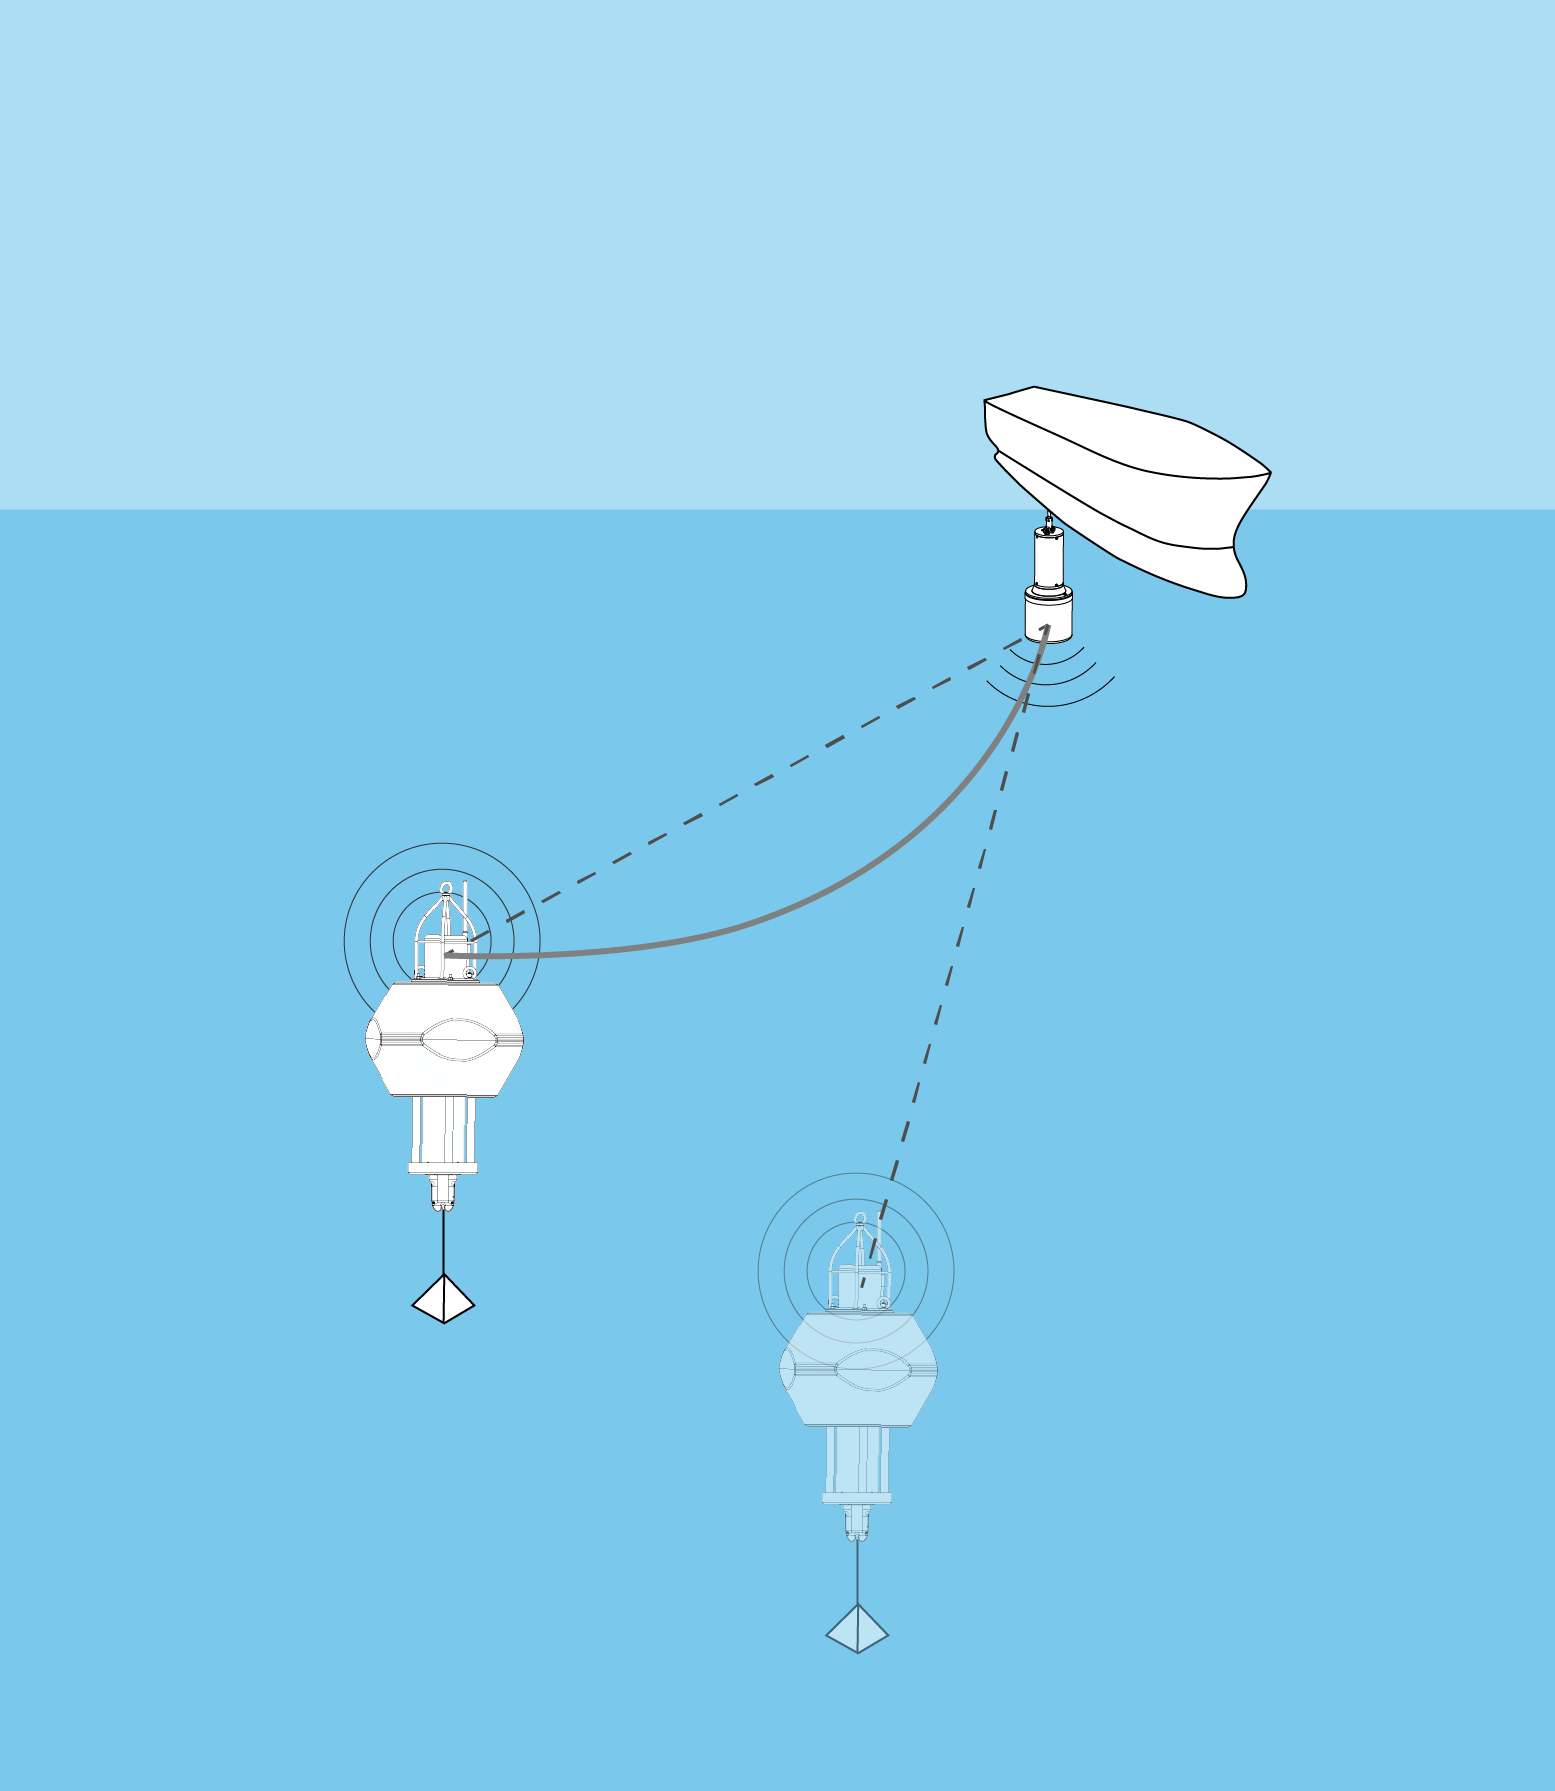
\includegraphics[width=0.8\textwidth]{ray-bending.png}
    \caption{Ray bending demo}
\end{figure}

To compensate this error several techniques can be used. In postprocessing an
Acoustic Tooklit (BELLHOP) can be used. It is too heavy to run it in real-time.

But some additional information can improve accuracy of measurements.
If transponder and USBL-transceiver depths below surface are known a vertical
part of waveform direction can be corrected.

Let $[ N, E, D ]^{T}$ -- motion-compensated coordinates in USBL-frame, $H_{t}$ --
depth below surface of target and $H_{u}$ -- depth below surface of
USBL-transceiver. Slant range to the target is $L = \sqrt{N^2 + E^2 + D^2}$,
horizontal range to target is $R = \sqrt{N^2 + E^2}$. Actual value of vertical
coordinate is $D^{'} = H_{t} - H_{u}$.

Since distance computation error is relative small, assume that it measured
correctly and correct horizontal coordinates to conform known depth and slant range.
Corrected horizontal range is:
\begin{equation}
    R^{'} = \sqrt{L^2 - (D^{'})^2} \\
\end{equation}

Coordinates correction is applied by:
\begin{equation}
    \begin{bmatrix}
        N^{'} \\ E^{'}
    \end{bmatrix} = \begin{bmatrix}
        N \\ E
    \end{bmatrix} \cdot \frac{R^{'}}{R}
\end{equation}


\section{Code examples}

\lstset{language=Matlab,frame=single}
\lstinputlisting{../lib/rpy2dcm.m}
\lstinputlisting{../lib/dcm2rpy.m}
\lstinputlisting{../lib/rpy2quat.m}
\lstinputlisting{../lib/quat2rpy.m}
\lstinputlisting{../lib/dcm2quat.m}
\lstinputlisting{../lib/quat2dcm.m}
\lstinputlisting{../lib/wgs84.m}
\lstinputlisting{../lib/get_n.m}
\lstinputlisting{../lib/geod2ecef.m}
\lstinputlisting{../lib/ecef2geod.m}
\lstinputlisting{../lib/geod2dcm.m}

\end{document}
